\documentclass[crop=false]{standalone}
%\documentclass{standalone}
\usepackage{tikz} % To generate the plot from csv
\usepackage{pgfplots}
\usepackage{graphicx}
\usepackage{booktabs}
\usepackage{subfig}
\usepackage{float}
\usepackage[section]{placeins} % getting figures below sections
\usepackage{blindtext}
\usepackage{siunitx}
\usepgfplotslibrary{units} % Allows to enter the units nicely
\usetikzlibrary{external} %https://tex.stackexchange.com/questions/1460/script-to-automate-externalizing-tikz-graphics
\tikzexternalize[prefix=savedfigures/]

\pgfplotsset{compat=newest} % Allows to place the legend below plot
\usepackage{pgfplotstable}
\usepgfplotslibrary{statistics}

% #################### Function definition for box plots read table ##################\
\makeatletter
\pgfplotsset{
	boxplot prepared from table/.code={
		\def\tikz@plot@handler{\pgfplotsplothandlerboxplotprepared}%
		\pgfplotsset{
			/pgfplots/boxplot prepared from table/.cd,
			#1,
		}
	},
	/pgfplots/boxplot prepared from table/.cd,
	table/.code={\pgfplotstablecopy{#1}\to\boxplot@datatable},
	row/.initial=0,
	make style readable from table/.style={
		#1/.code={
			\pgfplotstablegetelem{\pgfkeysvalueof{/pgfplots/boxplot prepared from table/row}}{##1}\of\boxplot@datatable
			\pgfplotsset{boxplot/#1/.expand once={\pgfplotsretval}}
		}
	},
	make style readable from table=lower whisker,
	make style readable from table=upper whisker,
	make style readable from table=lower quartile,
	make style readable from table=upper quartile,
	make style readable from table=median,
	make style readable from table=average,
	make style readable from table=lower notch,
	make style readable from table=upper notch
}
\makeatother
\begin{document}
\pgfkeys{/pgf/number format/.cd,1000 sep={\,}}

\section{21 2 Mumford0 SA Initial solutions 20210812 163415}

% ######################## UTRP SA Import saved solutions ######################## 
\begin{figure} 
\centering 
\tikzsetnextfilename{UTRP_DBMOSA_BP_initial_solutions} 
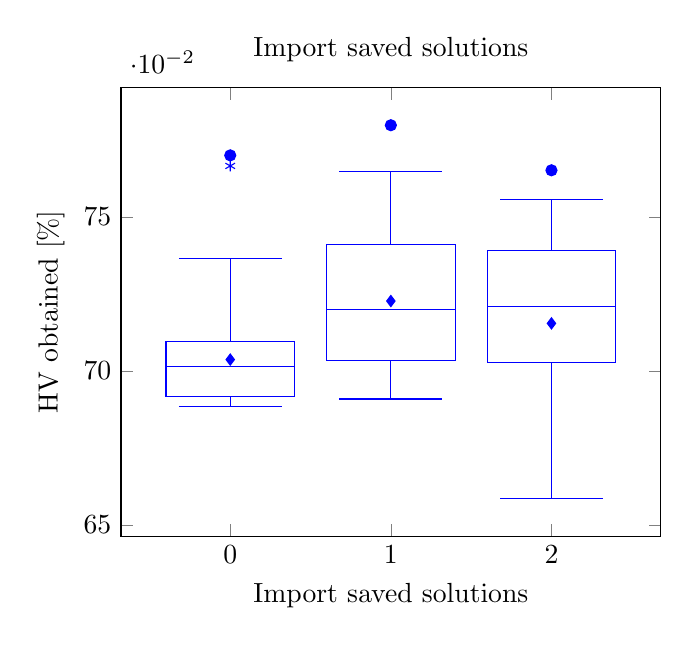
\begin{tikzpicture} 
\begin{axis}[ 
title={Import saved solutions}, 
boxplot/draw direction=y, 
xtick={1,2,3}, 
xticklabels={0,1,2}, 
x tick label style={rotate=0, align=center}, 
xlabel={Import saved solutions}, 
% y tick label style={/pgf/number format/.cd,fixed,precision=3, zerofill}, 
scaled y ticks={base 10:2}, 
ylabel={HV obtained [\%]}, 
] 

% ############## Choice_import_saved_set=0 ################## 
\addplot[boxplot, mark=asterisk, 
boxplot prepared={ 
lower whisker=0.68857, 
upper whisker=0.73639, 
lower quartile=0.6918, 
upper quartile=0.70962, 
median=0.70144, 
average=0.7037}, 
color = blue, solid, area legend] 
coordinates {
(1,0.76658)}; 
\addplot[only marks,mark=*,color = blue]coordinates{(1,0.77001)}; 

% ############## Choice_import_saved_set=1 ################## 
\addplot[boxplot, mark=asterisk, 
boxplot prepared={ 
lower whisker=0.69092, 
upper whisker=0.76477, 
lower quartile=0.70331, 
upper quartile=0.74114, 
median=0.72003, 
average=0.72272}, 
color = blue, solid, area legend] 
coordinates {}; 
\addplot[only marks,mark=*,color = blue]coordinates{(2,0.77979)}; 

% ############## Choice_import_saved_set=2 ################## 
\addplot[boxplot, mark=asterisk, 
boxplot prepared={ 
lower whisker=0.65849, 
upper whisker=0.75582, 
lower quartile=0.70275, 
upper quartile=0.73905, 
median=0.72083, 
average=0.71545}, 
color = blue, solid, area legend] 
coordinates {}; 
\addplot[only marks,mark=*,color = blue]coordinates{(3,0.76516)}; 

\end{axis}
\end{tikzpicture}
\end{figure} 

% ######################## UTRP SA Use supplemented initial solution set ######################## 
\begin{figure} 
\centering 
\tikzsetnextfilename{UTRP_DBMOSA_BP_initial_solutions} 
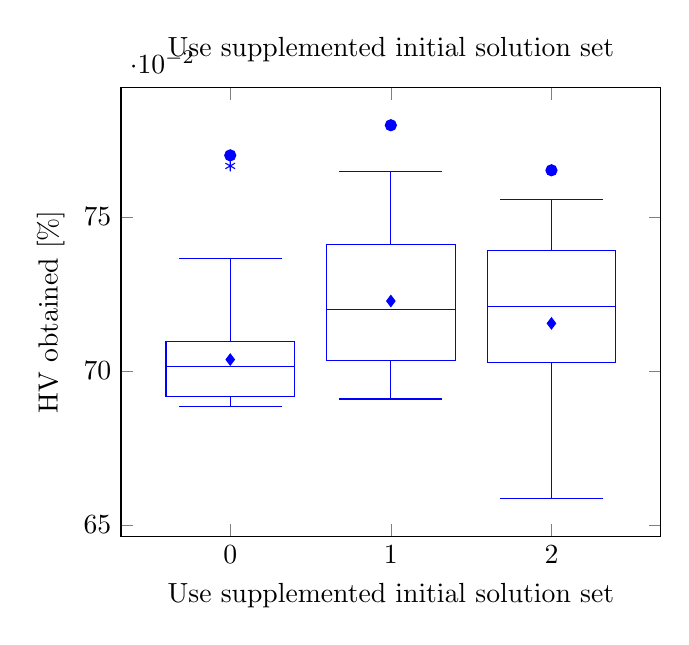
\begin{tikzpicture} 
\begin{axis}[ 
title={Use supplemented initial solution set}, 
boxplot/draw direction=y, 
xtick={1,2,3}, 
xticklabels={0,1,2}, 
x tick label style={rotate=0, align=center}, 
xlabel={Use supplemented initial solution set}, 
% y tick label style={/pgf/number format/.cd,fixed,precision=3, zerofill}, 
scaled y ticks={base 10:2}, 
ylabel={HV obtained [\%]}, 
] 

% ############## Initial_solutions=0 ################## 
\addplot[boxplot, mark=asterisk, 
boxplot prepared={ 
lower whisker=0.68857, 
upper whisker=0.73639, 
lower quartile=0.6918, 
upper quartile=0.70962, 
median=0.70144, 
average=0.7037}, 
color = blue, solid, area legend] 
coordinates {
(1,0.76658)}; 
\addplot[only marks,mark=*,color = blue]coordinates{(1,0.77001)}; 

% ############## Initial_solutions=1 ################## 
\addplot[boxplot, mark=asterisk, 
boxplot prepared={ 
lower whisker=0.69092, 
upper whisker=0.76477, 
lower quartile=0.70331, 
upper quartile=0.74114, 
median=0.72003, 
average=0.72272}, 
color = blue, solid, area legend] 
coordinates {}; 
\addplot[only marks,mark=*,color = blue]coordinates{(2,0.77979)}; 

% ############## Initial_solutions=2 ################## 
\addplot[boxplot, mark=asterisk, 
boxplot prepared={ 
lower whisker=0.65849, 
upper whisker=0.75582, 
lower quartile=0.70275, 
upper quartile=0.73905, 
median=0.72083, 
average=0.71545}, 
color = blue, solid, area legend] 
coordinates {}; 
\addplot[only marks,mark=*,color = blue]coordinates{(3,0.76516)}; 

\end{axis}
\end{tikzpicture}
\end{figure} 
\begin{table}
\centering
\caption{Legend for the boxplot.}
\begin{tabular}{ll}
\toprule
 Index &  Name \\
\midrule
     0 & False \\
     1 &  True \\
\bottomrule
\end{tabular}
\end{table}

\end{document}
